In order to achieve better discrimination between the Higgs boson signal and the SM backgrounds
compared to simple cuts we employ a Matrix Element technique. 
This method has already been used in top quark mass and cross-section 
measurements, the discovery of single top production, and Higgs boson searches at the Tevatron.  
The Matrix Element method works by calculating the probability for each recorded
event to originate from a specific physics process.
This is done by comparing the measured kinematic observables with the predicted
differential cross section given by a Matrix Element calculation
as a function of those observables for the signal and background processes.
The discriminating power arises because the differential cross sections for 
signal and background events are largest in different regions of the available
kinematic phase space. 
%In the Matrix Element approach we calculate the probability for each
%In this method 
%event to have originated from a specific physics process, using the measured kinematic 
%information from the event.  
%Probabilities are calculated based on the predicted differential
%cross section for the process.  

One complication of the Higgs to $WW$ leptonic final state is that it is not fully 
reconstructed, with two neutrinos in the final state. 
Information about the $z$-components of the neutrino momenta as well as the individual 
neutrino transverse components are missing. It is therefore necessary to integrate 
over these unknown quantities, which we perform using the importance sampling 
integration method.
%Since some of the kinematic information is
%missing due to the two neutrinos in the final state, we integrate over the missing
%information in the calculation of the differential cross section.
The Matrix Element functions used in the determination of the differential cross sections
for this analysis are obtained from  MCFM v5.8.  While MCFM 
provides both leading order (LO) and next-to leading (NLO) cross-section calculations for 
all relevant background and Higgs processes in $pp$ collisions, only the
LO is currently used.

The probabilities for all processes under consideration are combined 
to construct a single discriminant, called the Likelihood Ratio (LR).  
To construct the optimal discriminant, one should calculate 
event probabilities for all of the background processes. In reality, however, having 
probabilities for the signal hypothesis and the main backgrounds is sufficient for the 
desired level of discrimination. In this analysis we calculate event probabilities 
for gluon fusion Higgs boson production ($ggH$), electroweak $q\bar{q}\rightarrow WW$ pair 
production ($WW$) and the $W+jet$ process where a $W$ boson is produced in association with one hadronic jet. 
%In the future we plan to add ME calculations for other backgrounds such as for examples 
%$t\bar t$.


\subsection{Event Probability Calculation}

In the Matrix Element technique we calculate a probability  for each event assuming a
certain hypothesis.  The probability is denoted by $P(x_{obs};\alpha)$,
where $\alpha$ is a set of physics 
parameters of the specific model and $x_{obs}$ are the measured kinematic quantities.
In the case of Standard Model Higgs Boson production,
 $\alpha$ is $(m_H, \Gamma_H)$, where  $m_H$ is the Higgs mass 
and $\Gamma_H$ is the Higgs width. There are eight observables, $x_{obs}$, representing all the 
lepton kinematic information: lepton momenta $\vec{l}^+$, $\vec{l}^-$ and missing 
transverse momentum, \met$_x$ and \met$_y$.

It should be noted that additional information such as the number of jets
produced and the total visible energy might further differentiate the Higgs signal from SM
$WW$ production,
but they can suffer from significant  QCD uncertainties. For this reason we 
deliberately do not use hadronic information at all but use
only the kinematic information from the leptons and the missing $E_T$.

The event probability density is given by
\begin{equation}
P(x_{obs};\alpha) =
 {1 \over < \sigma(\alpha) > }
 \int \frac {d \sigma_{0} (y;\alpha) }{ dy }
 \epsilon (y) G(x_{obs},y) dy,  
\label{eqn:EvtProb}  
\end{equation}
where $y$ denotes the true values of the observables,
$d \sigma_{LO} \over  dy$ is the  parton-level differential cross-section differential
in those observables, $\epsilon(y)$ is the detector acceptance and efficiency function
and $G(x_{obs},y)$ is the transfer function between the true and measured values of the
observables, representing the detector resolution.
Equation (\ref{eqn:EvtProb}) integrates over all possible true values of the
observables, $y$, consistent with the measured quantities $x_{obs}$.
The constant $<\sigma(\alpha)>$ normalizes the total event probability to unity
%, i.e.
%\begin{equation}
%\int_{x_{obs}\in V_{acceptance}} { P ( x_{obs}; \alpha)  d x_{obs} } = 1.
%\end{equation}
and is equal to the LO cross-section ($\sigma_{LO}$) times the acceptance.
%One complication of the Higgs to $WW$ leptonic final state is that it is not fully 
%reconstructed. Information about $z$-components of neutrino momenta as well as individual 
%neutrino transverse components are missing. It is, therefore, necessary to integrate 
%over these unknown quantities which we do using importance sampling integration method.

%\subsubsection{Efficiency Function}
The efficiency function is the probability for a parton-level object with momentum 
$p$ to be reconstructed as a lepton with momentum $q$. In the calculation of the event 
probabilities we assume that the parton level lepton momentum is equal to the reconstructed 
momentum. The lepton efficiency is parameterized as a function of transverse momentum and 
pseudo-rapidity and extracted from $WW$ Monte Carlo. Figure~\ref{fig:lepeff_gen} shows the 
one dimensional projection of the efficiency as a function of the lepton $\eta$ and $\pt$. 
A scale factor to account for
differences between data and Monte Carlo can be calculated using a tag-and-probe analysis 
and applied when calculating event probabilities for data events. 

Note that the efficiency function in Equation~\ref{eqn:EvtProb} can be factorized out of
the integral when calculating event probabilities.
%The efficiency function in Equation~\ref{eqn:EvtProb} can be pulled out from 
%the integral when calculating event probabilities, for example in the case of $WW$ process:
%\begin{eqnarray}
%\begin{array}{lcl}
%P_{WW}(x_{obs};\alpha) & = &
% \frac{\epsilon (\eta_{1,obs})\epsilon (\eta_{2,obs})}{ < \sigma_{WW} > }
% \int \frac {d \sigma_{WW} (y;\alpha) }{ dy }
%  G(x_{obs},y) dy. \\
%\end{array} 
%\end{eqnarray}

%%%%%%%%%%%%%%%%%%%%%%%%%%%%%%
\begin{figure}[!htbp]
\begin{center}
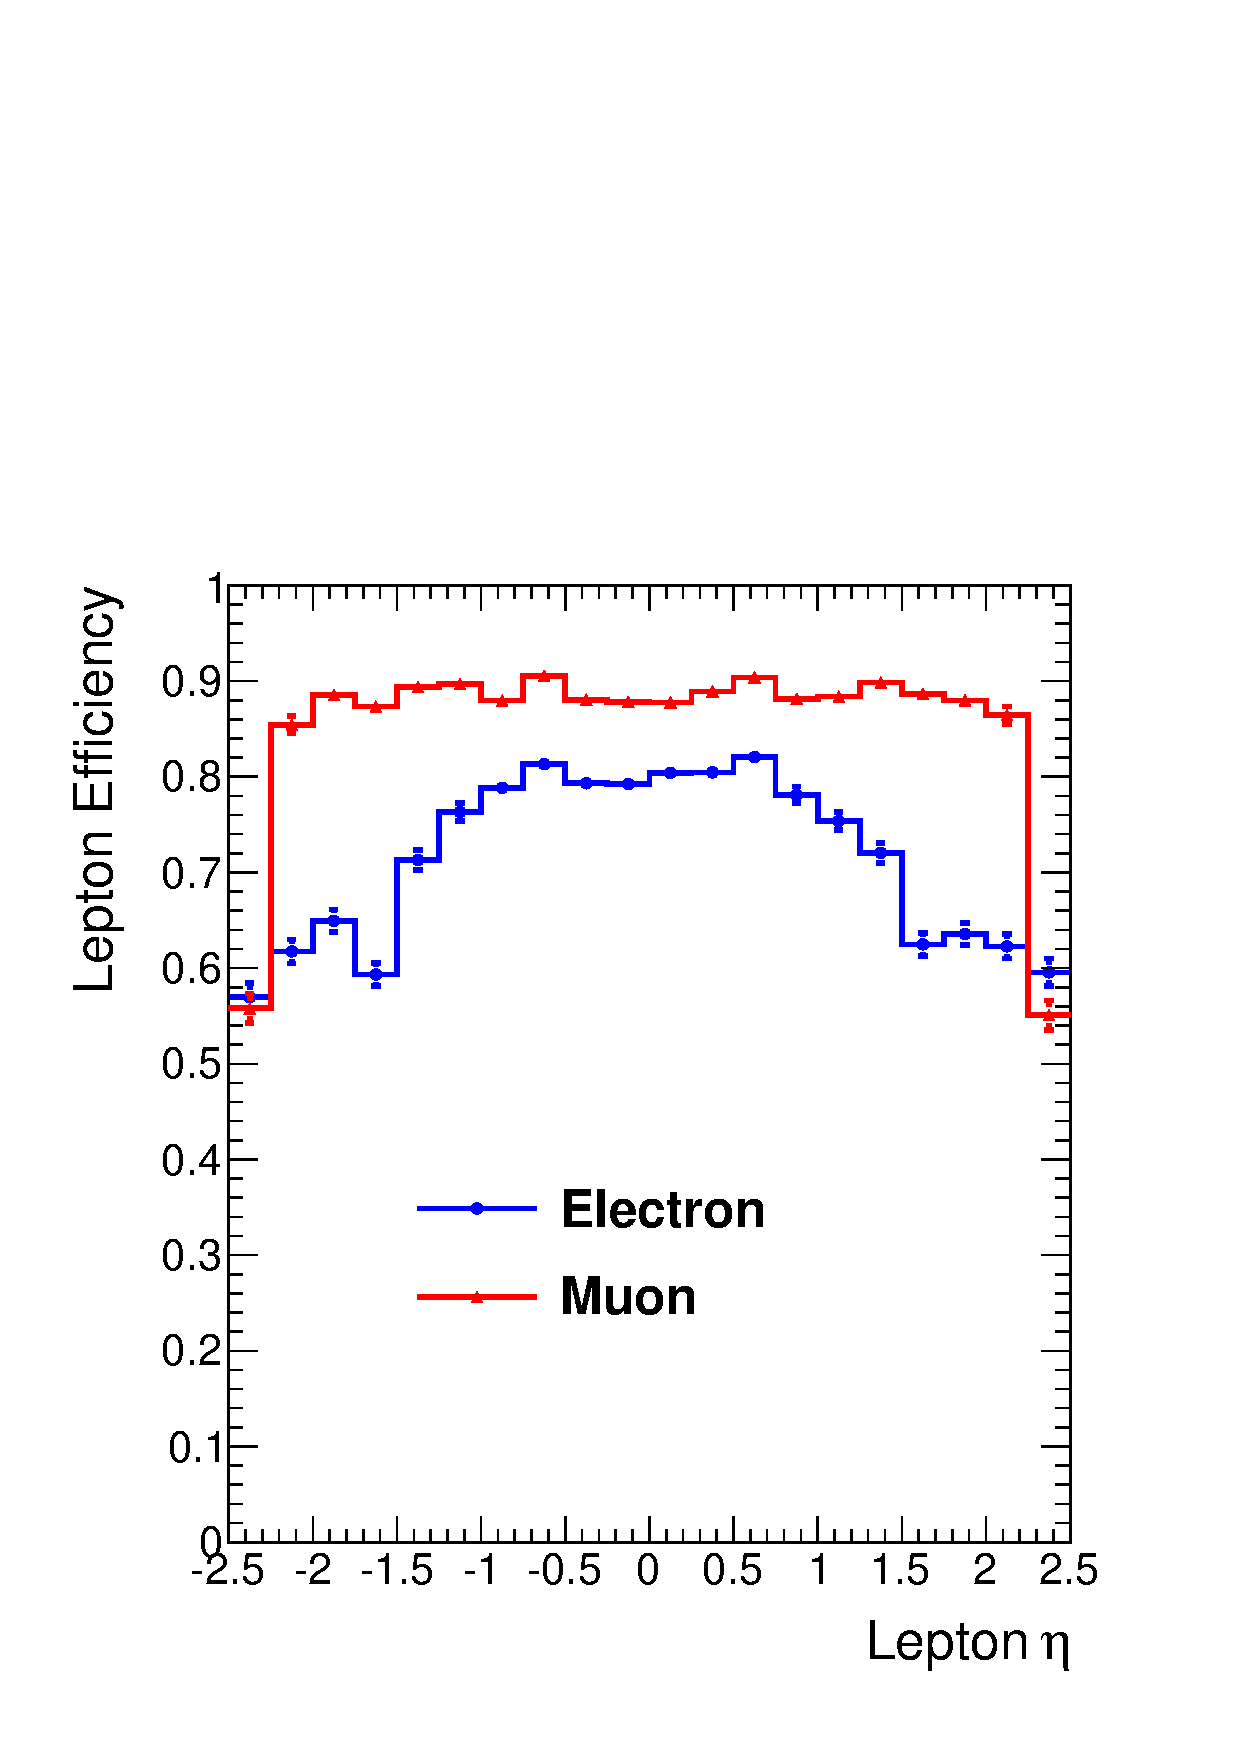
\includegraphics[width=0.4\textwidth]{figures/lepton_eff_Eta.pdf}
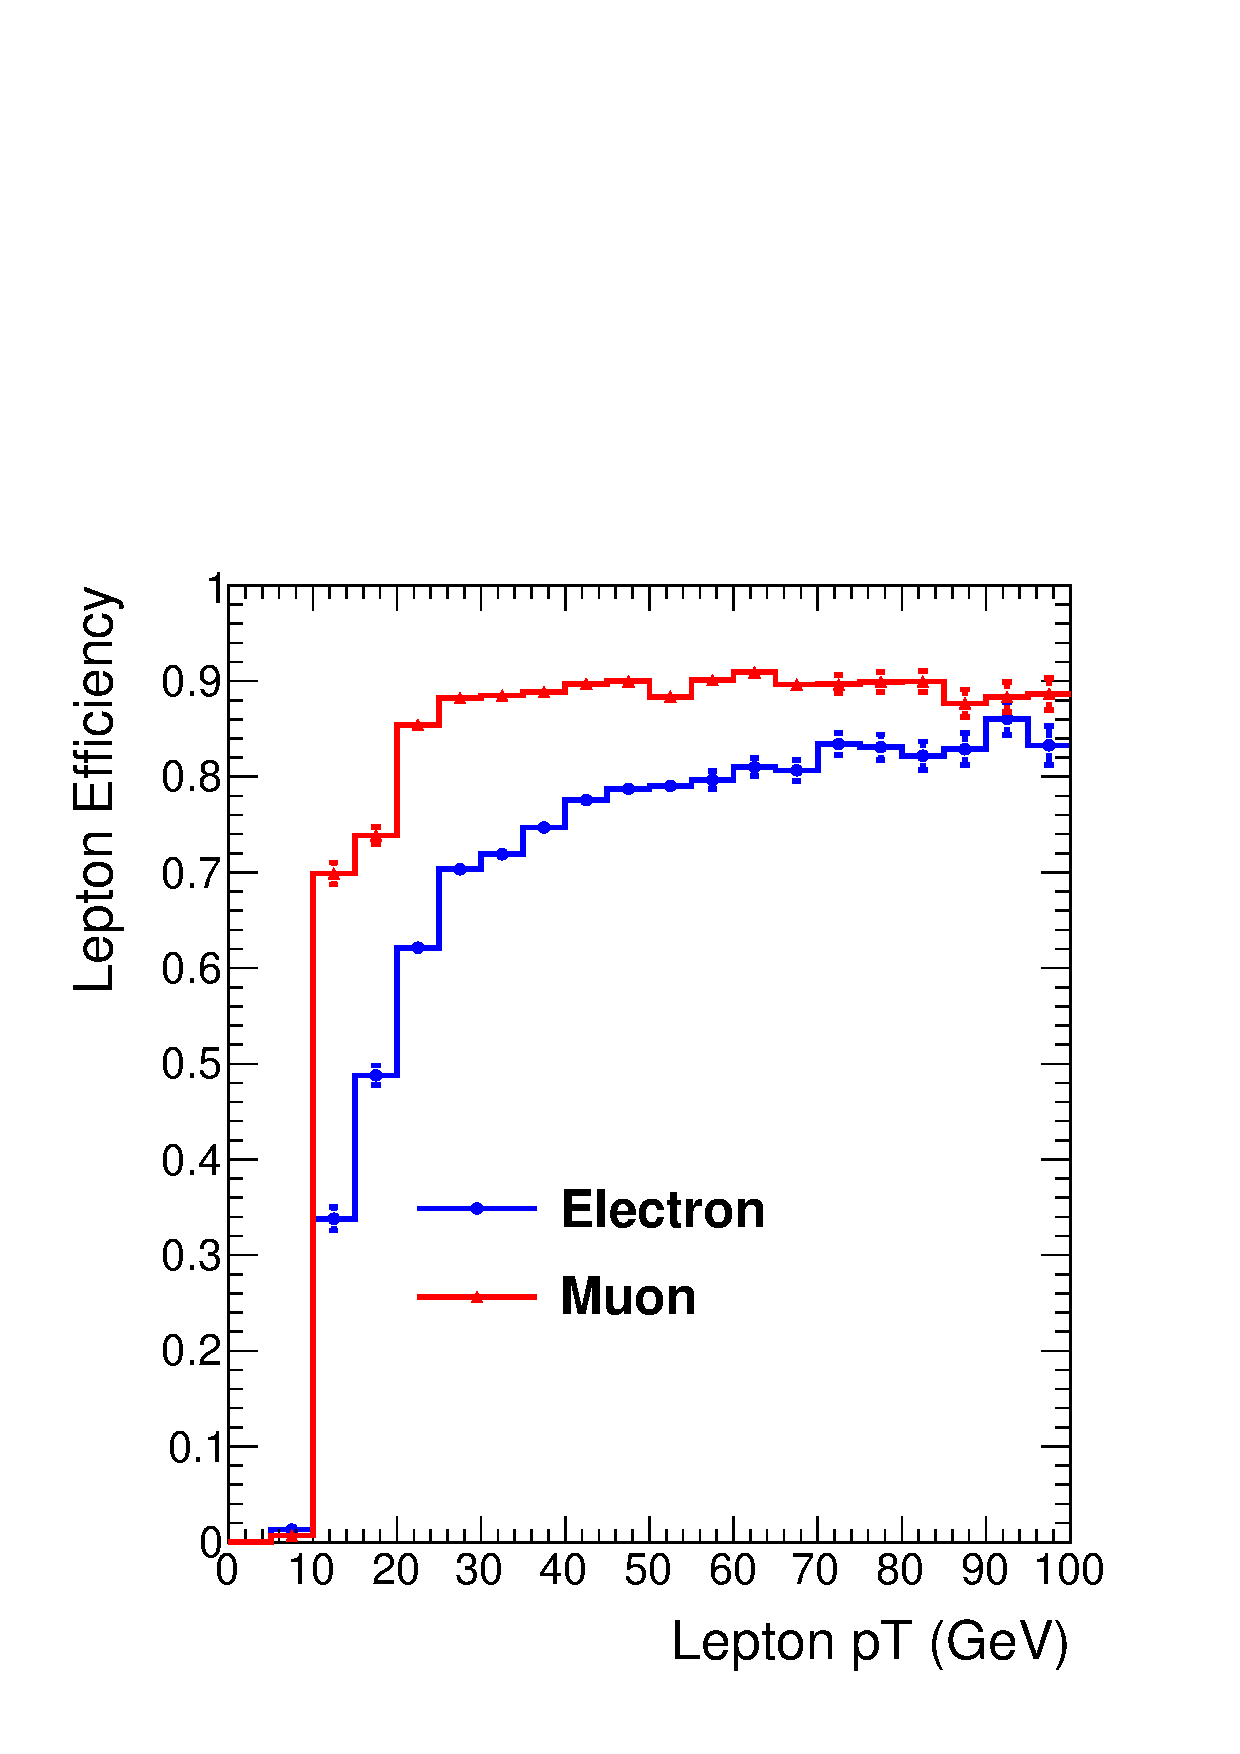
\includegraphics[width=0.4\textwidth]{figures/lepton_eff_Pt.pdf}\\
\caption{Lepton efficiency as a function of the lepton $\eta$ (left) and $\pt$ (right) extracted 
from the $\WW$ Monte Carlo.}
\label{fig:lepeff_gen}
\end{center}
\end{figure}
%%%%%%%%%%%%%%%%%%%%%%%%%%%%%%




Treatment of the $W+jet$ event probability calculation deserves special discussion.
For these events to be reconstructed in the dilepton final state,
one of the reconstructed leptons has been faked by a parton fragmenting and hadronizing 
into a QCD jet which then fakes the signature of a lepton in the detector. To account for this 
effect properly, we multiply the differential cross-section for the $W+jet$ process by the 
probability for a parton to be reconstructed as a lepton with the measured kinematics. 
This probability can be factorized into two terms:
\begin{eqnarray}
\begin{array}{lcl}
P(parton\rightarrow lepton)=P(parton\rightarrow FO)\times P(FO\rightarrow lepton)
\end{array} 
\end{eqnarray} 
where FO refers to a so-called "fakeable object" (see Sec.~\ref{sec:bkg_fakes}). 
The first term in the product is measured using Monte Carlo and parametrized
in $p_{T}$ and $\eta$.  The second term is the fake rate measured in the data 
(see Sec.~\ref{sec:bkg_fakes}).

We verify the $P(parton\rightarrow lepton)$ values we obtain from this method by comparing them to ones measured in a $\gamma+jet$ Monte Carlo sample.  The probabilities agree within the uncertainty of $30\%$.  The values of $P(parton\rightarrow lepton)$ are illustrated in Figure~\ref{fig:lepgenfr}.

%%%%%%%%%%%%%%%%%%%%%%%%%%%%%%
\begin{figure}[!htbp]
\begin{center}
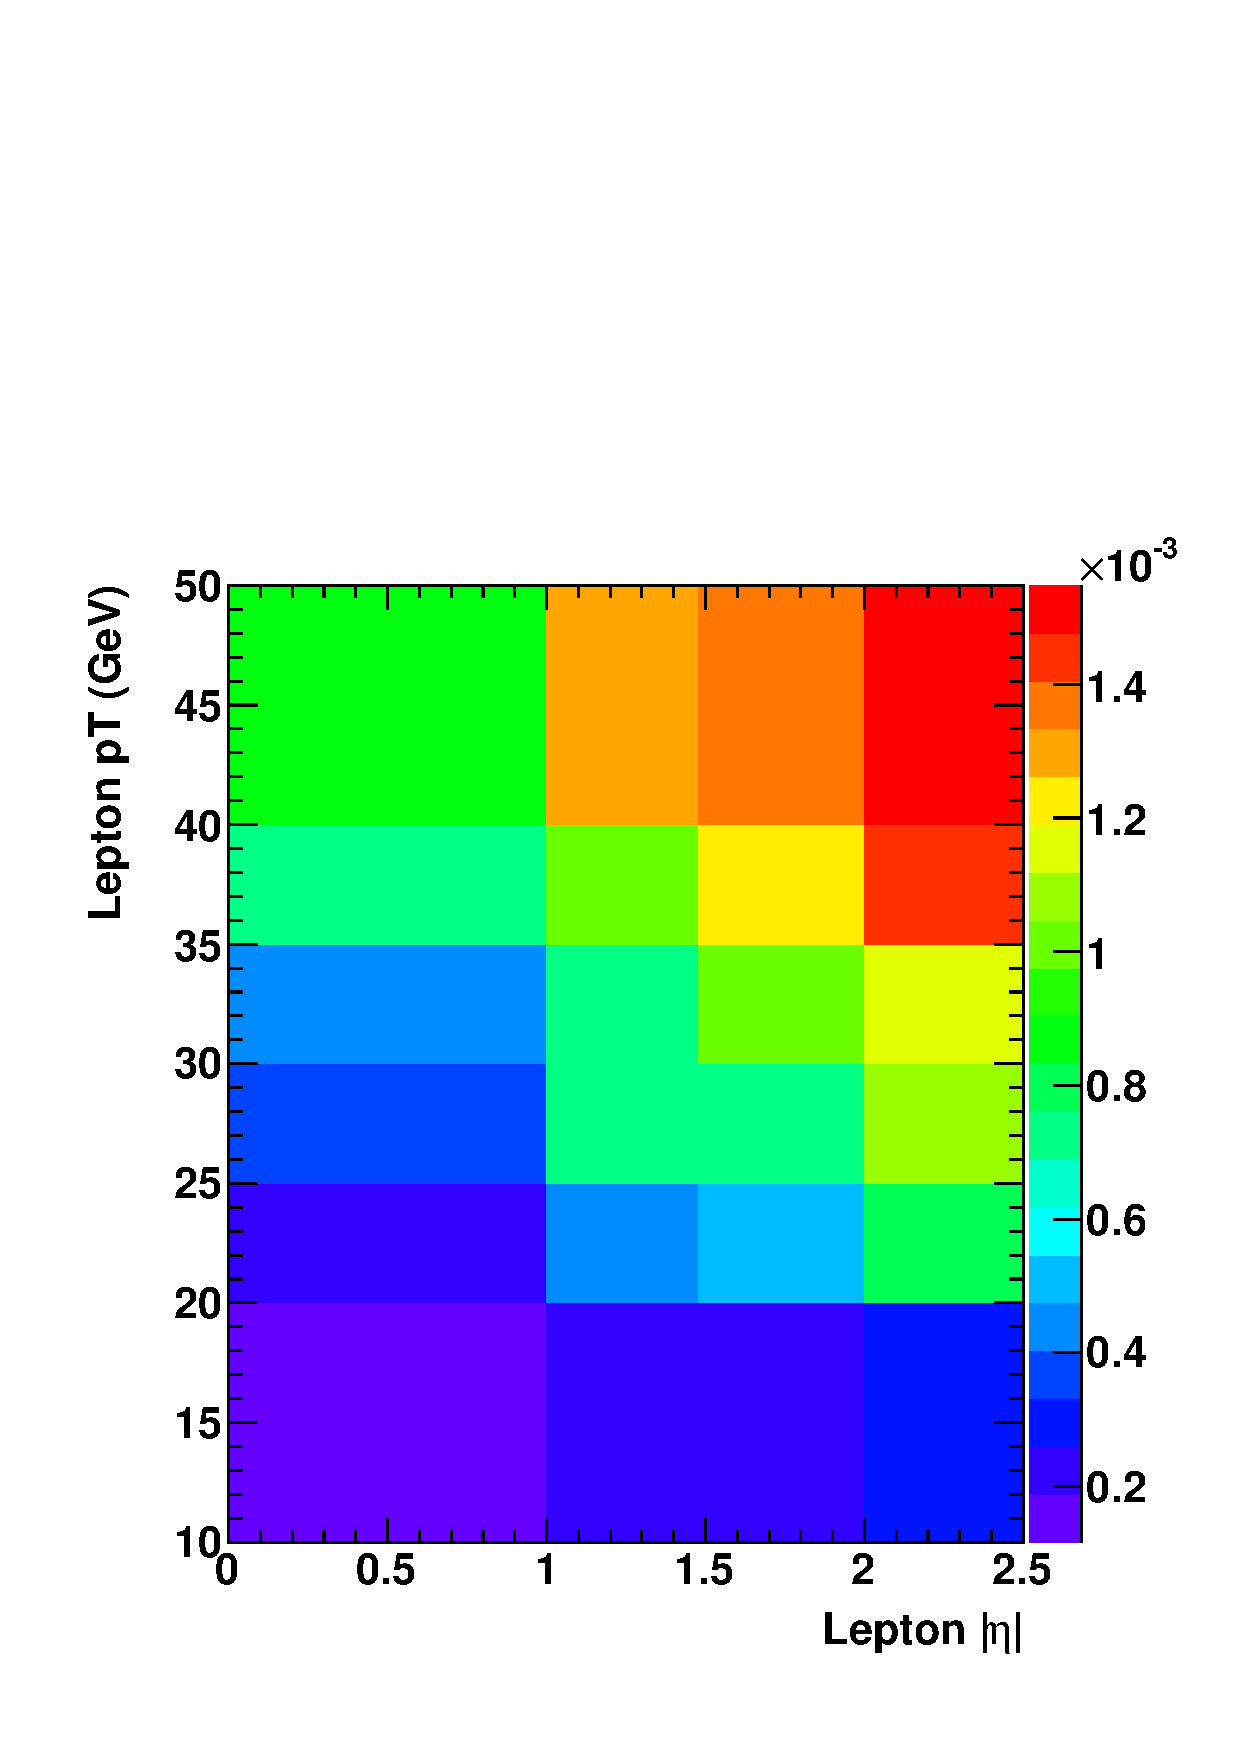
\includegraphics[width=0.4\textwidth]{figures/wjets_heleGenFR.pdf}
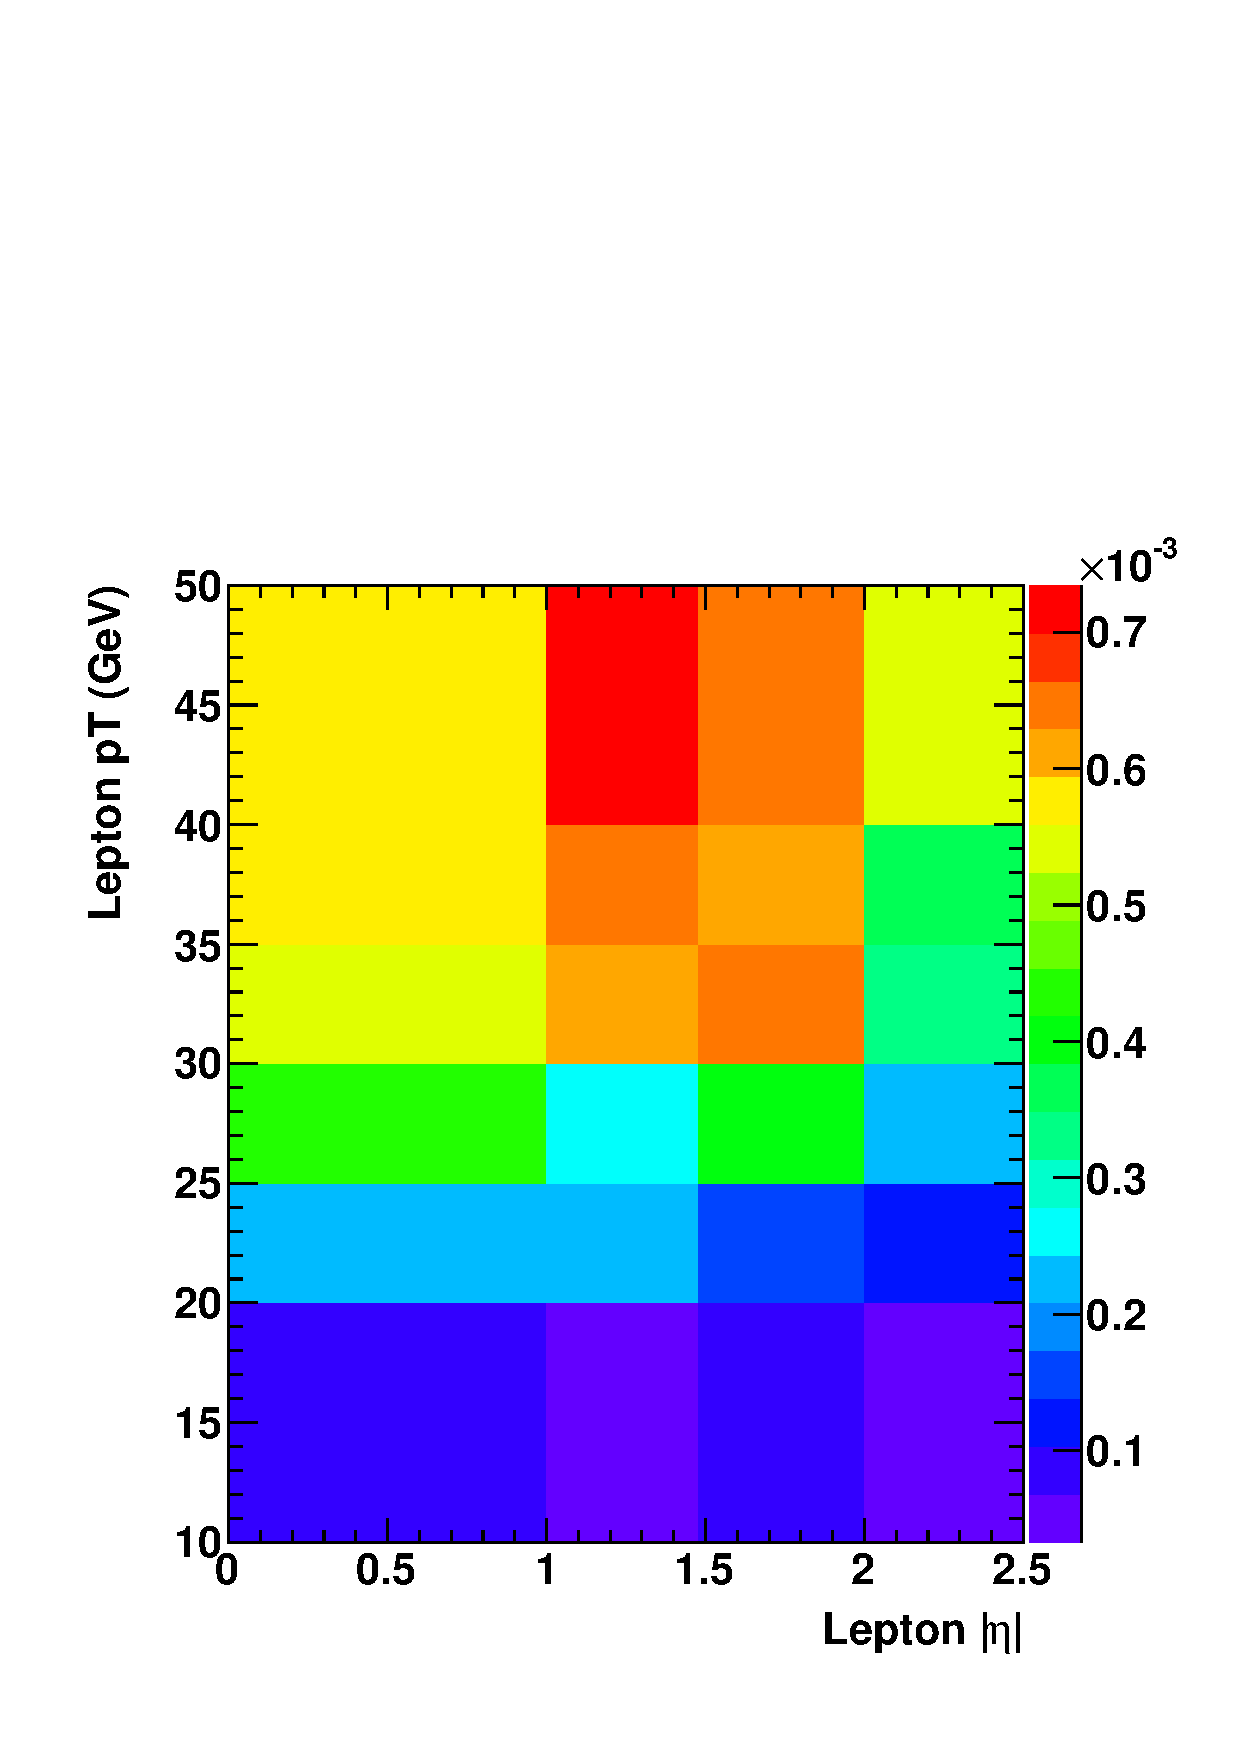
\includegraphics[width=0.4\textwidth]{figures/wjets_hmuGenFR.pdf}\\
\caption{The probability for a parton to pass the electron (left) and muon (right) 
fakable object selections. }
\label{fig:lepgenfr}
\end{center}
\end{figure}
%%%%%%%%%%%%%%%%%%%%%%%%%%%%%%

%The $W+jet$ event probability can be then  written as:
%\begin{eqnarray}
%\begin{array}{lcl}
%P_{Wjet}(x_{obs};\alpha) & = &
% \frac{\epsilon(\eta_{1obs})\epsilon_{j\rightarrow D}(\eta_{2obs})
% \epsilon_{D\rightarrow l}(p_{T2,obs})}{ < \sigma_{W\text{jet}} > }
% \int \frac {d \sigma_{WW} (y;\alpha) }{ dy }
%  G(x_{obs},y) dy+ 1\leftrightarrow 2. \\
% \end{array} 
%\end{eqnarray}

%\subsubsection{{\bf $k_T$} Function}
One final complication that must be considered is the boost of the initial state.
In the leading order Matrix Element calculation there is no initial state radiation. 
The initial state partons collide head-on and the system has no transverse boost. 
To account for the transverse recoil and thus improve the performance of our discriminant
on data, we integrate over the possible values of the system boost $k_{T}(k_{x},k_{y})$. 
The $k_T$ model is extracted from Monte Carlo for each process separately. 
Figure~\ref{fig:wwboost} shows the distribution of $k_T$ for $\hww$ and 
the non-resonant $\WW$ processes.  


%%%%%%%%%%%%%%%%%%%%%%%%%%%%%%
\begin{figure}[!htbp]
\begin{center}
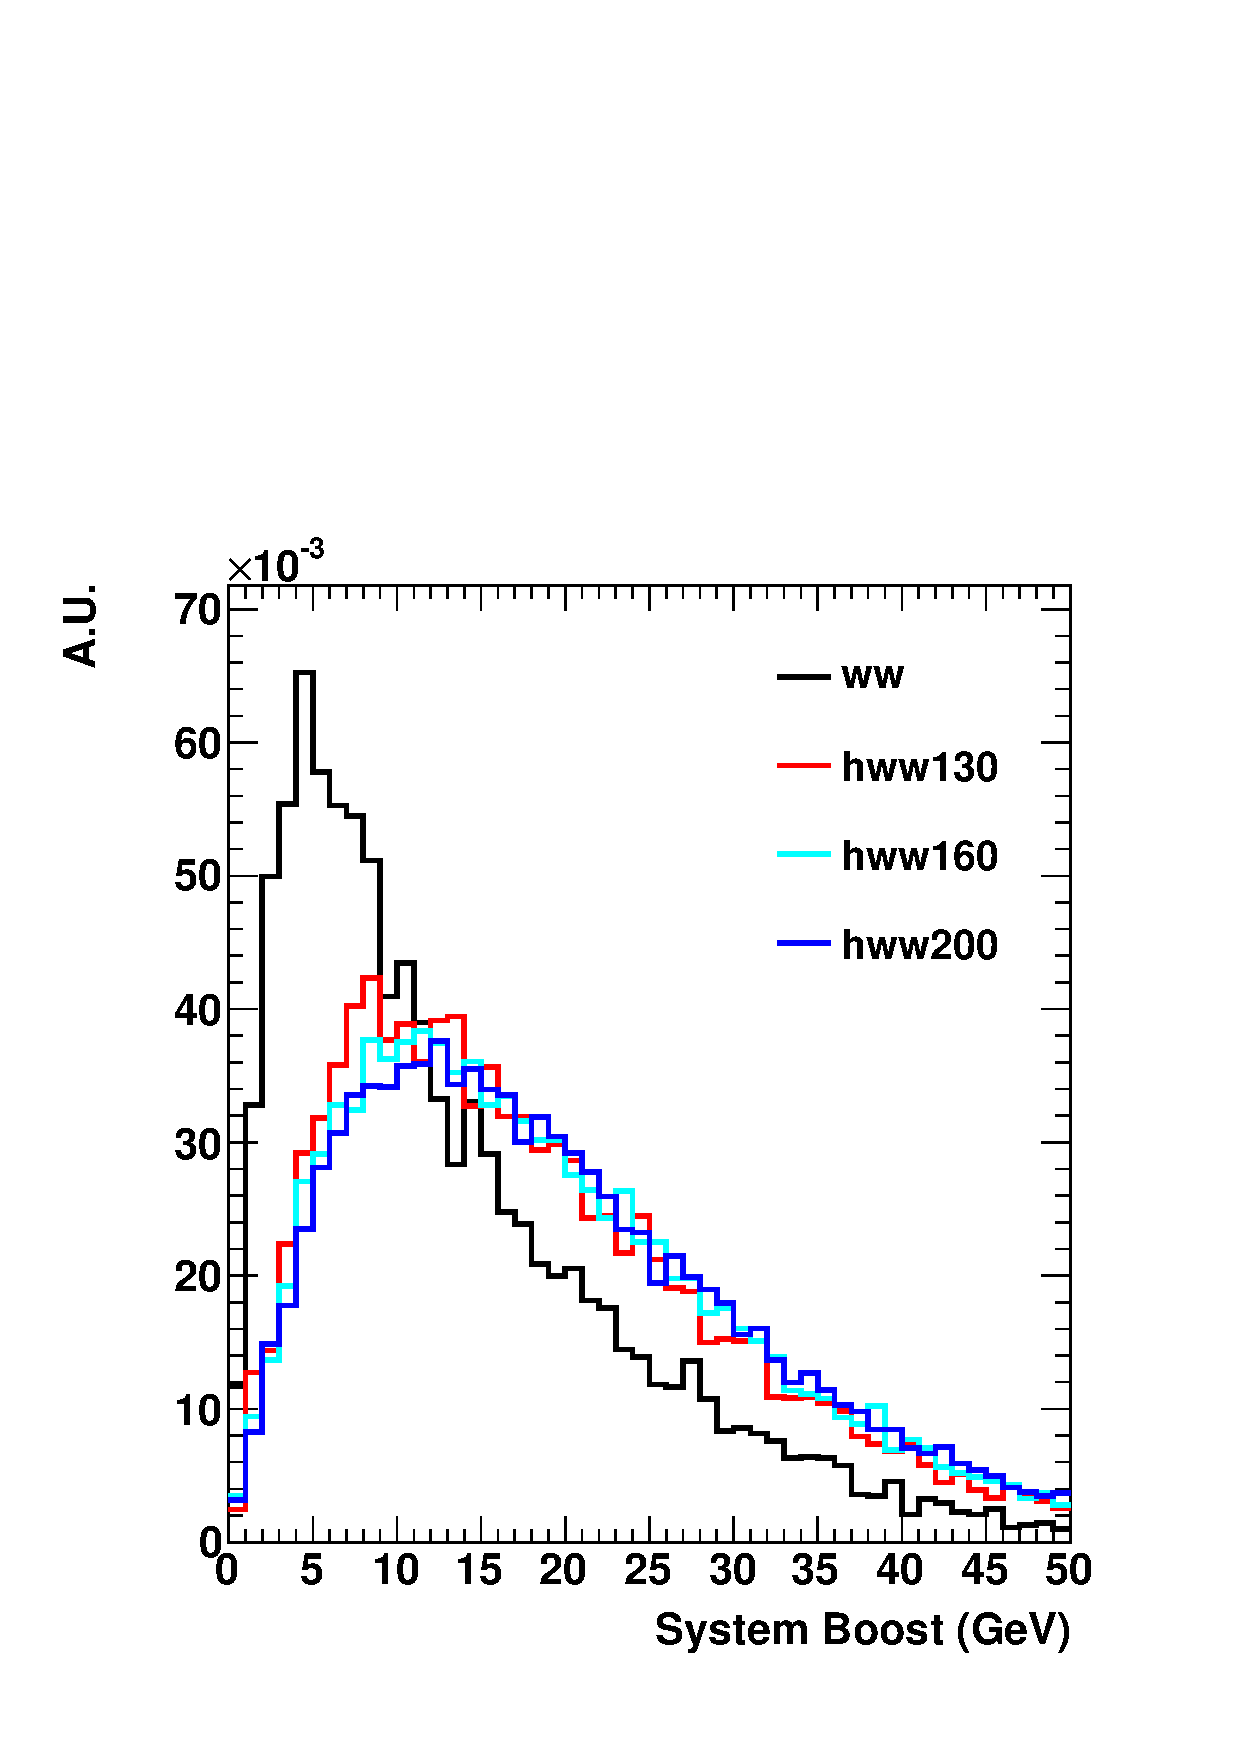
\includegraphics[width=0.5\textwidth]{figures/boost.pdf}
\caption{The transverse boost of the $WW$ system. }
\label{fig:wwboost}
\end{center}
\end{figure}
%%%%%%%%%%%%%%%%%%%%%%%%%%%%%%


\subsection{Likelihood Ratio Discriminator}
Event probabilities, calculated as described above, are used to construct 
a likelihood ratio discriminant which we use in a one-dimensional template fit.  
The discriminator is defined as :
\begin{equation}
\label{eqn:LR}
LR = \frac { P_s} { P_s + \sum_i k_{bi} P_{bi}},
\end{equation}
where $P_s$  is the probability for the signal, $P_{bi}$ is the probability for background
process $i$, and
$k_{bi}$ is the expected fractional contribution of background $i$,
satisfying the sum $\sum k_{bi} =1$.
Because signal events are expected to have $P_s>P_b$ and vice-versa for background events, 
the value of $LR$ is close to one for signal and zero for background processes.
The calculation of $P_s$ is a function of Higgs mass so that the likelihood ratio
shape depends on $m_H$. This is true for both signal and background templates of $LR$. 
Figure~\ref{fig:lrstacks} shows the likelihood ratio distributions for $m_H$~=~130, 160, and 200 $GeV/c^2$, 
corresponding to 1$\fb$. 
Note that the backgrounds peak near $LR~=~0$ while the signal peaks near $LR~=~1$. 
%%%%%%%%%%%%%%%%%%%%%%%%%%%%%%
\begin{figure}[!hbtp]
\centering
\subfigure[]{
\centering
\label{subfig:lr_hm130}
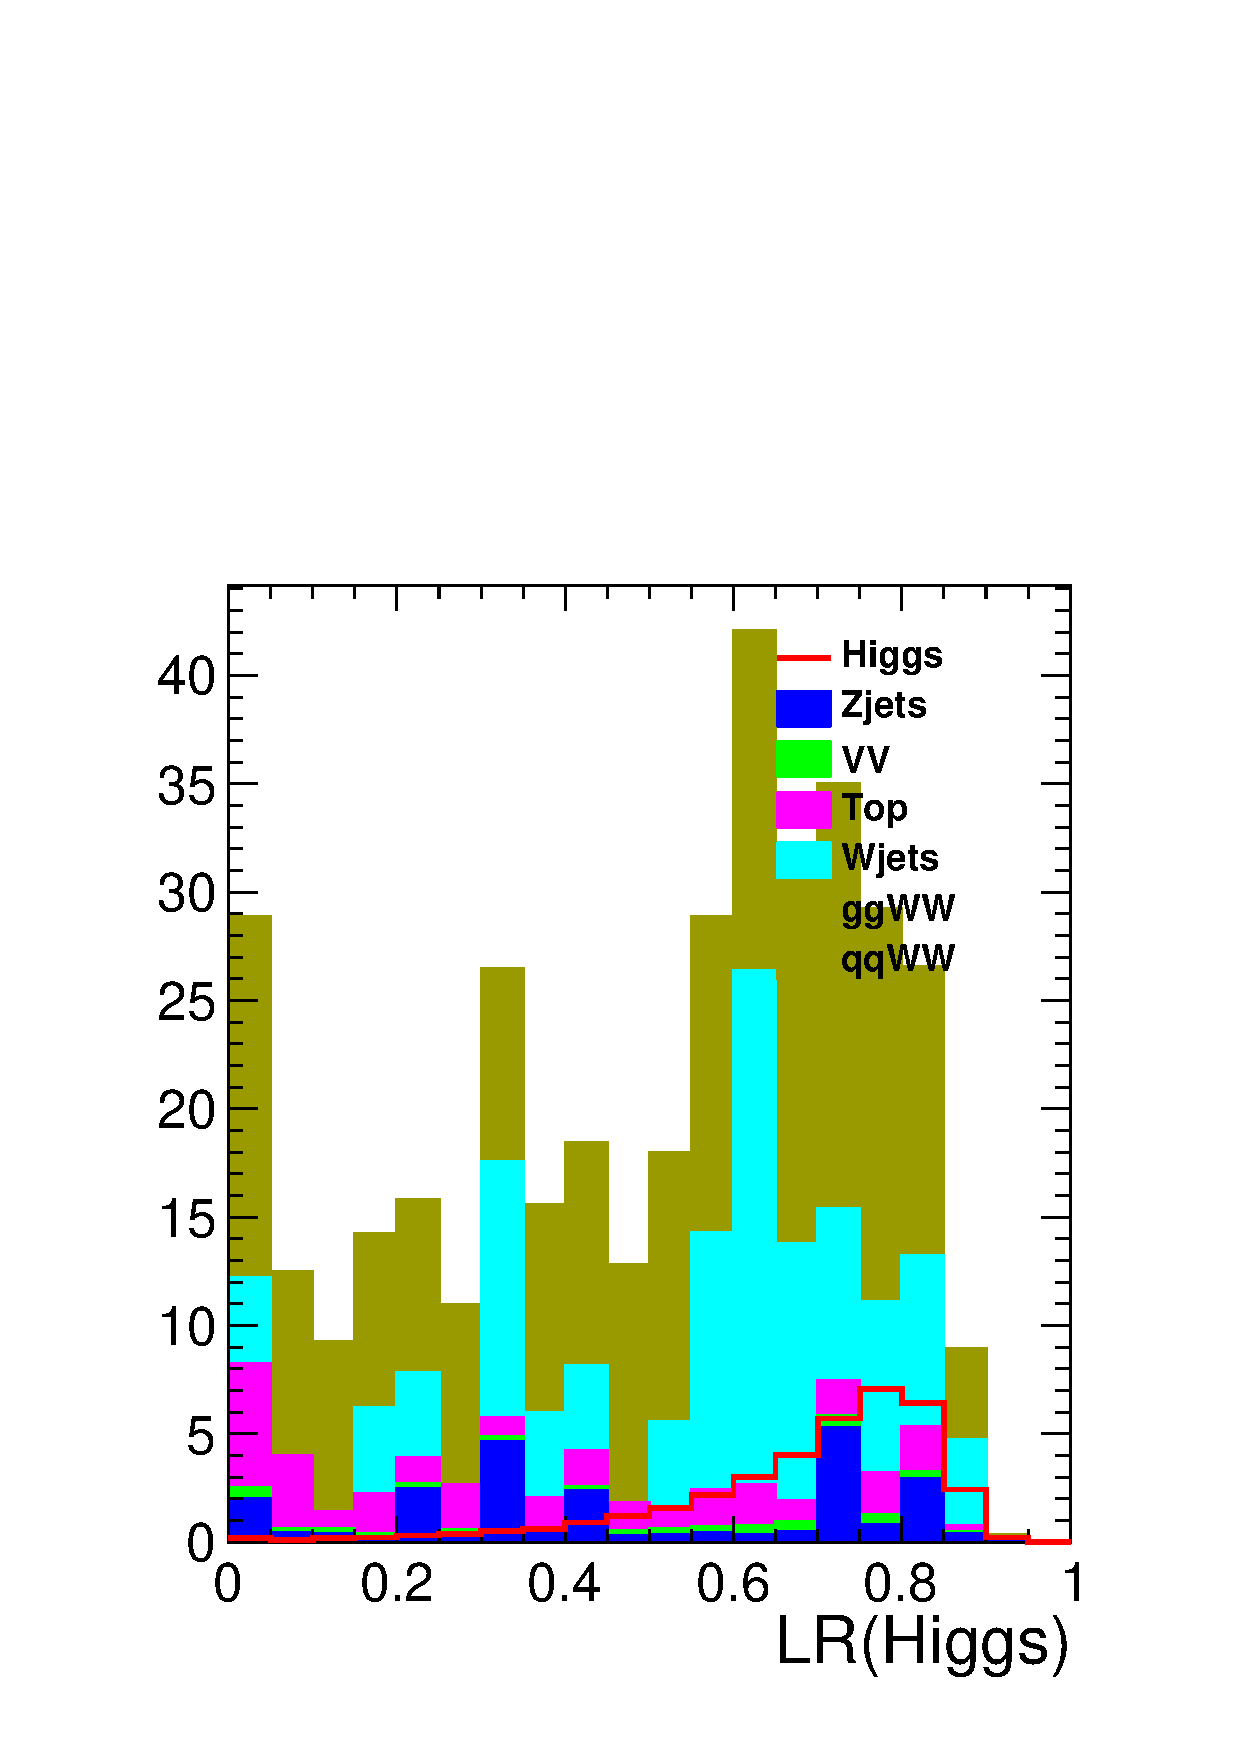
\includegraphics[width=.32\textwidth]{figures/hww130_LR.pdf}}
\subfigure[]{
\centering
\label{subfig:lr_hm160}
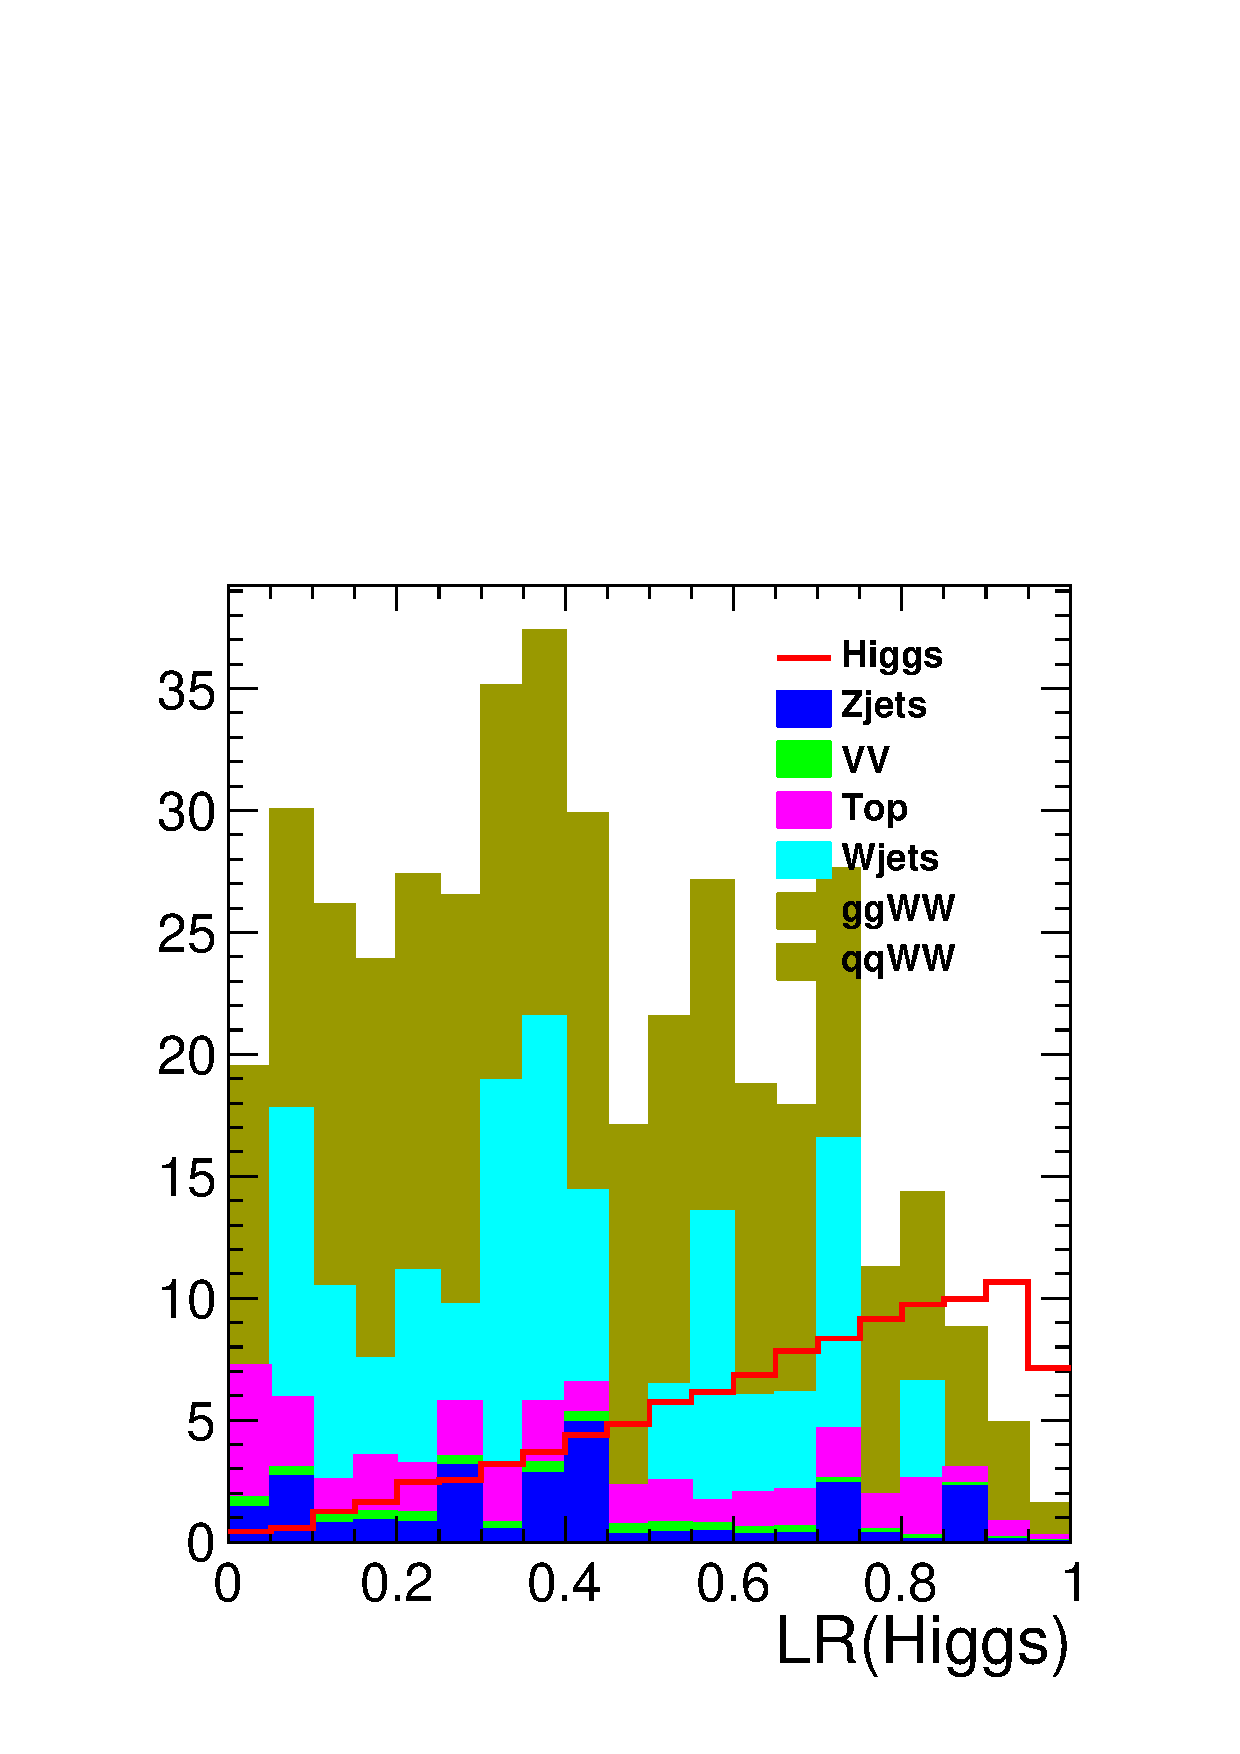
\includegraphics[width=.32\textwidth]{figures/hww160_LR.pdf}}
\subfigure[]{
\centering
\label{subfig:lr_hm200}
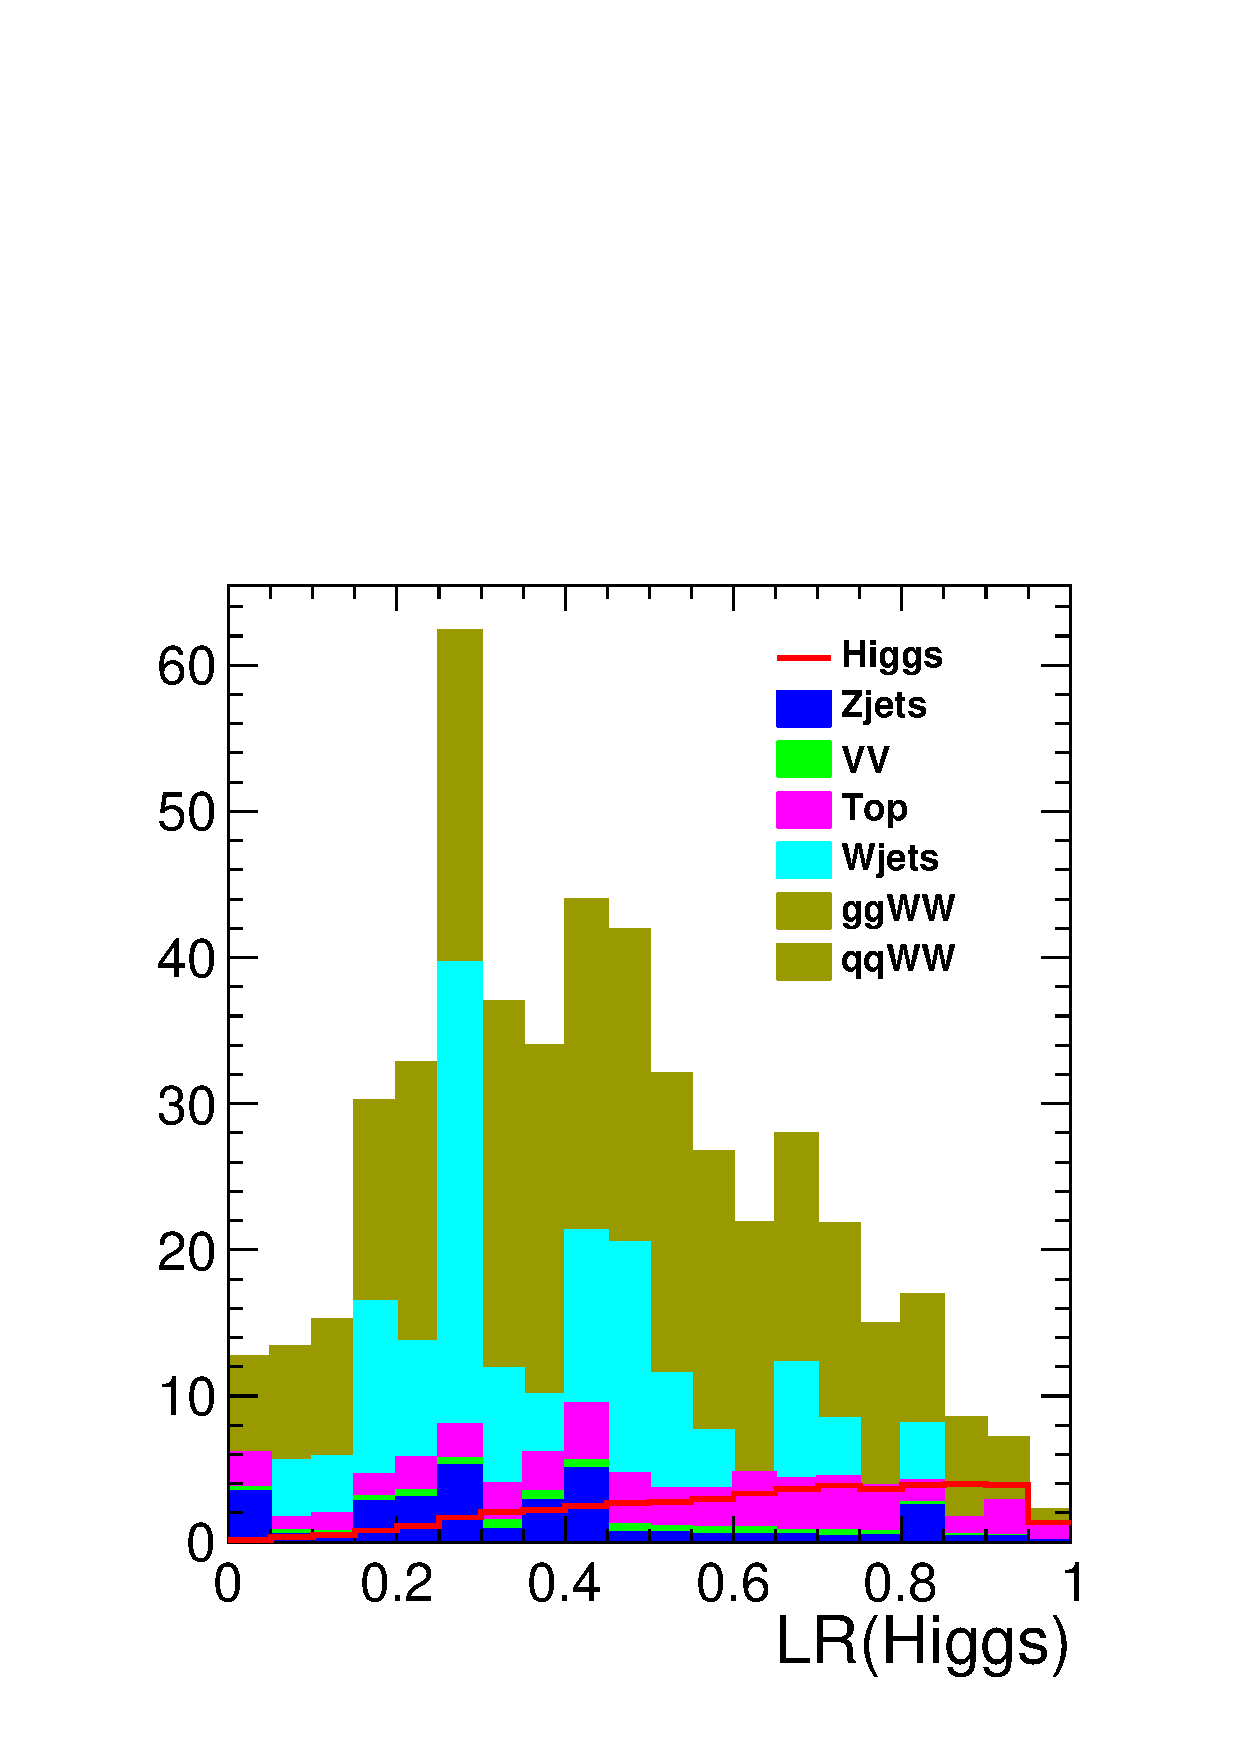
\includegraphics[width=.32\textwidth]{figures/hww200_LR.pdf}}\\
\caption{The matrix element output LR distribution after \WW\ selection and $m_{ll}$ cut 
for $m_H$=160 $\GeVcc$ \subref{subfig:lr_hm130}, $m_H$=160 $\GeVcc$ \subref{subfig:lr_hm160} 
and $m_H$=200 $\GeVcc$ \subref{subfig:lr_hm200} in the 0-jet bin.}
\label{fig:lrstacks}
\end{figure}
%%%%%%%%%%%%%%%%%%%%%%%%%%%%%%

It is important to note that because the $LR$ distribution is calculated the same way for data, 
signal and backgrounds, the fact that we use a LO Matrix Element and make certain 
approximations in the analytic calculation may result in less than optimal sensitivity 
%but does not introduce any mismodeling.
but does not introduce any bias.

\subsection{Sensitivity projection with 1$\fb$}

We compute the upper limits using the shape of the LR to maximize the analysis sensitivity as described in 
Section~\ref{sec:results}. The expected upper limit at 95\%C.L as a function of $m_H$ using the LR are shown in 
Figure~\ref{fig:me_expected_1fb} comparing the corresponding results using the BDT output. 
The sensitivity performance of the matrix element method is consistent with the BDT based approach, with a 
slightly larger exclusion region. 

%%%%%%%%%%%%%%%%%%%%%%%%%%%%%%
\begin{figure}[!hbtp]
\centering
\subfigure[]{
\centering
\label{subfig:me_exp_1fb}
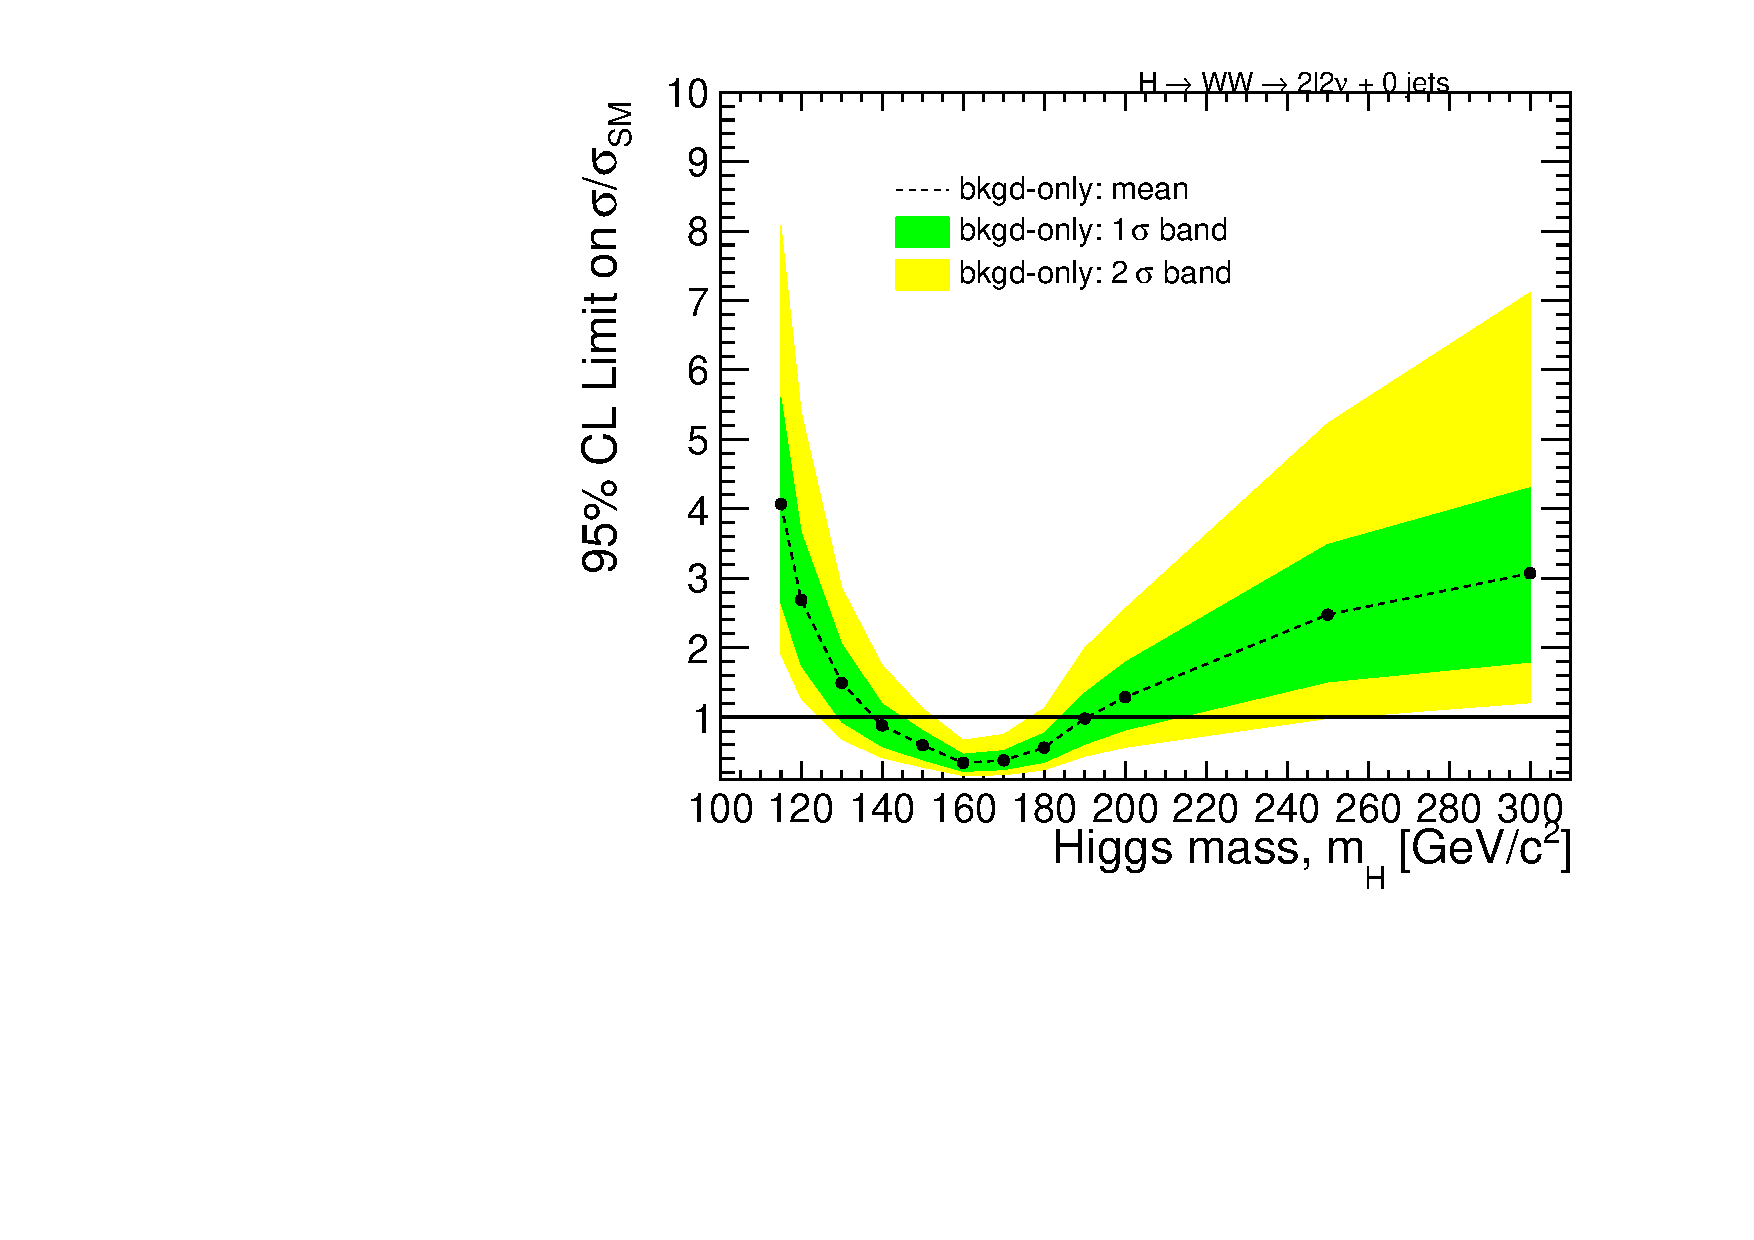
\includegraphics[width=.45\textwidth]{figures/limits_0j_1000pb_ME_shape.pdf}}
\subfigure[]{
\centering
\label{subfig:bdt_exp_1fb}
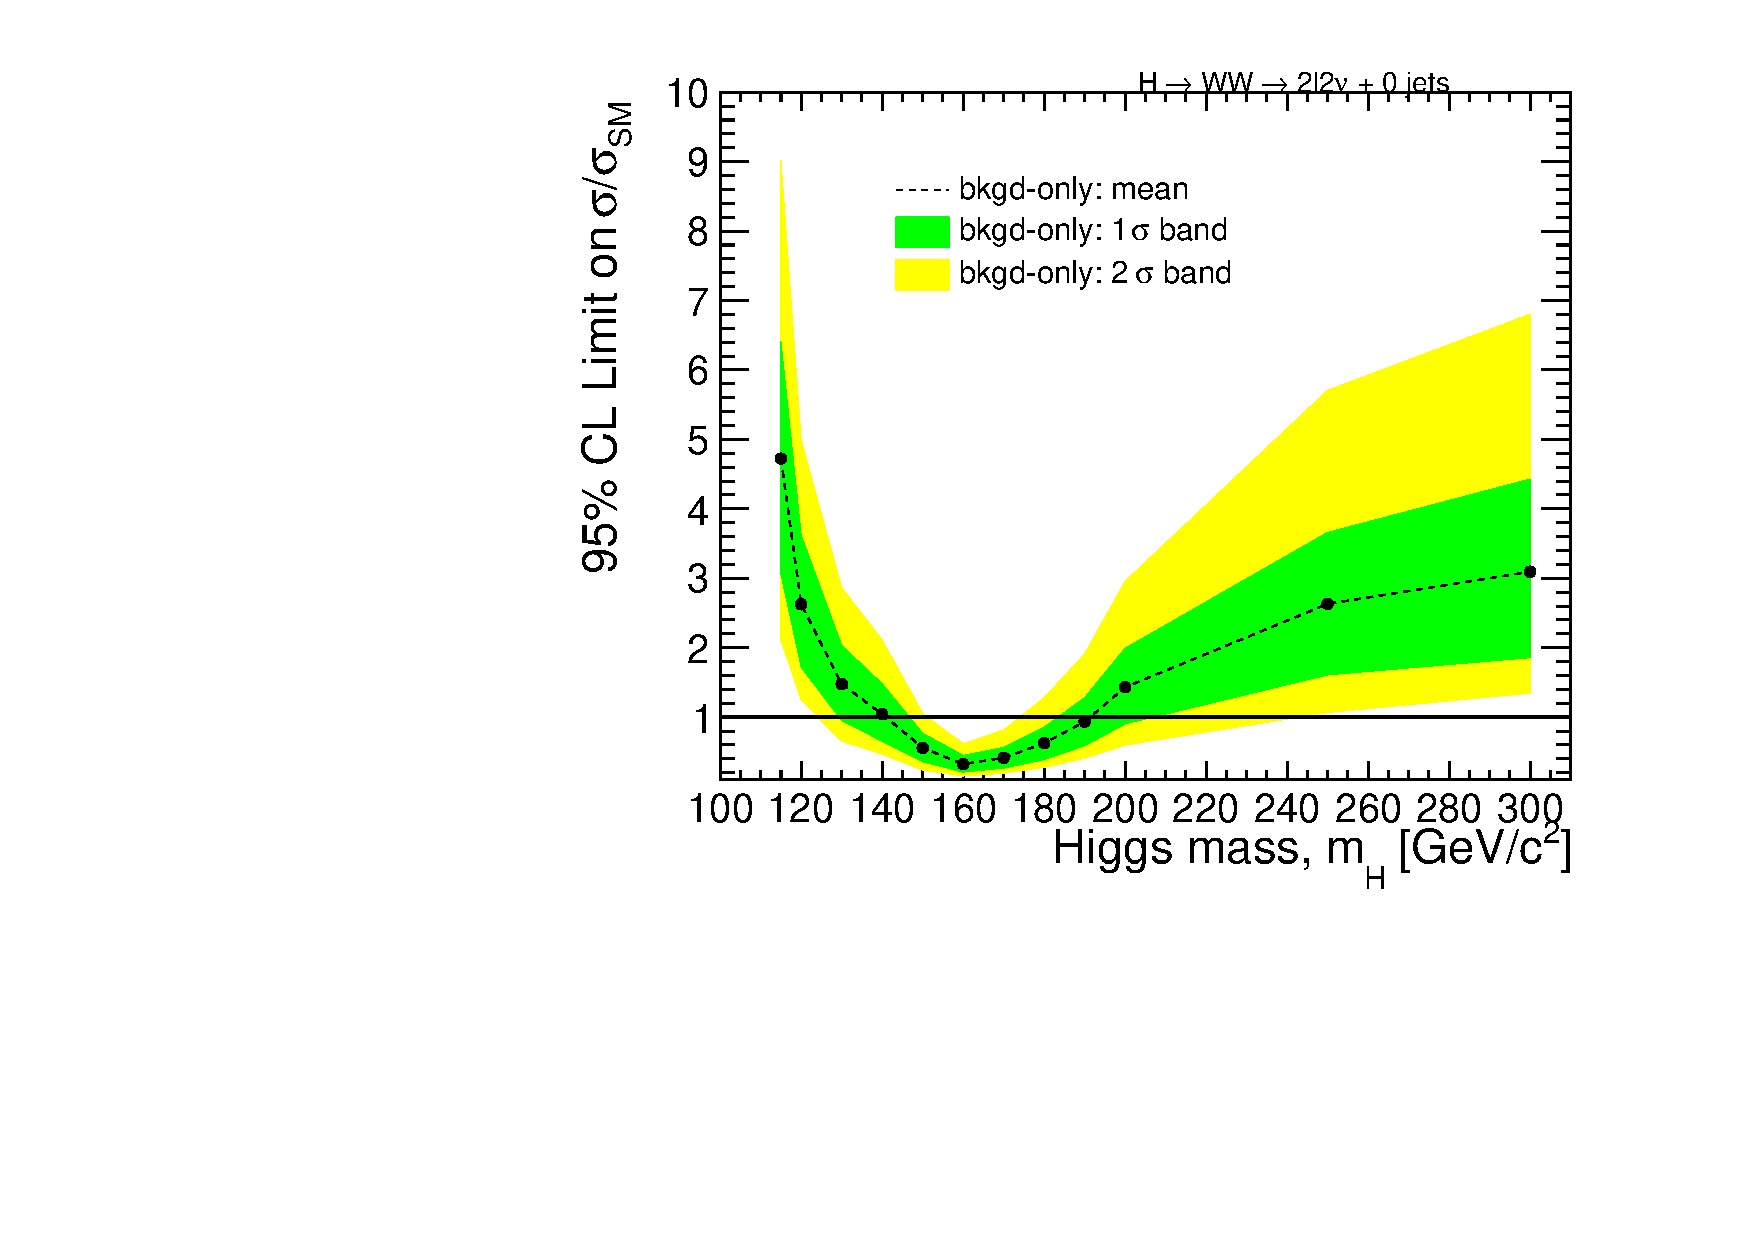
\includegraphics[width=.45\textwidth]{figures/limits_0j_1000pb_BDT_shape.pdf}} \\
\caption{ 
Multivariate shape analysis expected upper limits at 95\% C.L. for 1$\fb$ data using the 
matrix elemement output \subref{subfig:me_exp_1fb} and BDT output \subref{subfig:bdt_exp_1fb}. } 
\label{fig:me_expected_1fb}
\end{figure}
%%%%%%%%%%%%%%%%%%%%%%%%%%%%%%

%%%%%%%%%%%%%%%%%%%%%%%%%%%%%%
\begin{table}
\begin{center}
\begin{tabular}{c c c c c c c}
\hline\hline
 $m_H$ (GeV) & $-2\sigma$ & $-\sigma$ & mean & $+1\sigma$ & $+2\sigma$ \\
\hline
\multicolumn{6}{c} {Matrix Element Method} \\
\hline
115 & 1.90 &  2.64 &  4.07 &  5.60 & 8.08 \\
 120 & 1.27 &  1.75 &  2.69 &  3.66 & 5.39 \\
 130 & 0.68 &  0.93 &  1.49 &  2.05 & 2.86 \\
 140 & 0.42 &  0.58 &  0.88 &  1.19 & 1.75 \\
 150 & 0.28 &  0.39 &  0.60 &  0.81 & 1.12 \\
 160 & 0.16 &  0.22 &  0.34 &  0.47 & 0.67 \\
 170 & 0.17 &  0.24 &  0.38 &  0.52 & 0.75 \\
 180 & 0.24 &  0.35 &  0.56 &  0.77 & 1.13 \\
 190 & 0.44 &  0.61 &  0.98 &  1.35 & 1.99 \\
 200 & 0.57 &  0.81 &  1.29 &  1.79 & 2.56 \\
 250 & 0.98 &  1.51 &  2.48 &  3.49 & 5.23 \\
 300 & 1.21 &  1.79 &  3.07 &  4.30 & 7.11 \\
\hline
\multicolumn{6}{c} {BDT Based} \\
\hline
 115 & 2.11 &  3.06 &  4.72 &  6.40 & 9.01 \\
 120 & 1.25 &  1.72 &  2.63 &  3.62 & 4.99 \\
 130 & 0.66 &  0.95 &  1.48 &  2.03 & 2.86 \\
 140 & 0.47 &  0.65 &  1.04 &  1.48 & 2.11 \\
 150 & 0.24 &  0.36 &  0.56 &  0.77 & 1.05 \\
 160 & 0.15 &  0.21 &  0.32 &  0.45 & 0.62 \\
 170 & 0.19 &  0.27 &  0.42 &  0.57 & 0.81 \\
 180 & 0.28 &  0.39 &  0.63 &  0.85 & 1.28 \\
 190 & 0.41 &  0.59 &  0.93 &  1.28 & 1.91 \\
 200 & 0.60 &  0.90 &  1.43 &  1.99 & 2.96 \\
 250 & 1.07 &  1.61 &  2.63 &  3.66 & 5.71 \\
 300 & 1.35 &  1.86 &  3.09 &  4.43 & 6.80 \\
\hline\hline
\end{tabular}
\end{center}
\caption{Multivariate shape analysis expected upper limits at 95\% C.L. for 1$\fb$ data using the 
matrix elemement and BDT output corresponding to Figure~\ref{fig:me_expected_1fb}.}
\label{tab:me_expected_1fb}
\end{table}
%%%%%%%%%%%%%%%%%%%%%%%%%%%%%%